\documentclass{article}
\usepackage[T1]{fontenc}
\usepackage{lmodern}
\usepackage{graphicx}
\usepackage{amsmath,amssymb}
\usepackage[a4paper,margin=2cm]{geometry}
\usepackage[absolute,overlay]{textpos}
\setlength{\TPHorizModule}{1mm}
\setlength{\TPVertModule}{1mm}
\usepackage[indonesian]{babel}
\usepackage{hyperref}
\setlength{\emergencystretch}{2em}
% unit: Halaman 23

\begin{document}

% === Halaman 23 (llm) ===

% (tidak ada teks dari model)

% deskripsi: Screenshot Command Prompt Windows yang menunjukkan eksekusi program Caesar Cipher. Terlihat proses enkripsi teks 'the quick brown fox jumps over the lazy dog' dengan pergeseran 18 menjadi 'LZW IMAUC TJGOF XGP BMEHK GNWJ LZW DSRQ UGY', kemudian didekripsi kembali ke teks asli.
% bbox normalisasi: [0.0950, 0.1280, 0.9050, 0.8540]
\begin{textblock*}{170.10mm}(19.95mm,38.02mm)
\noindent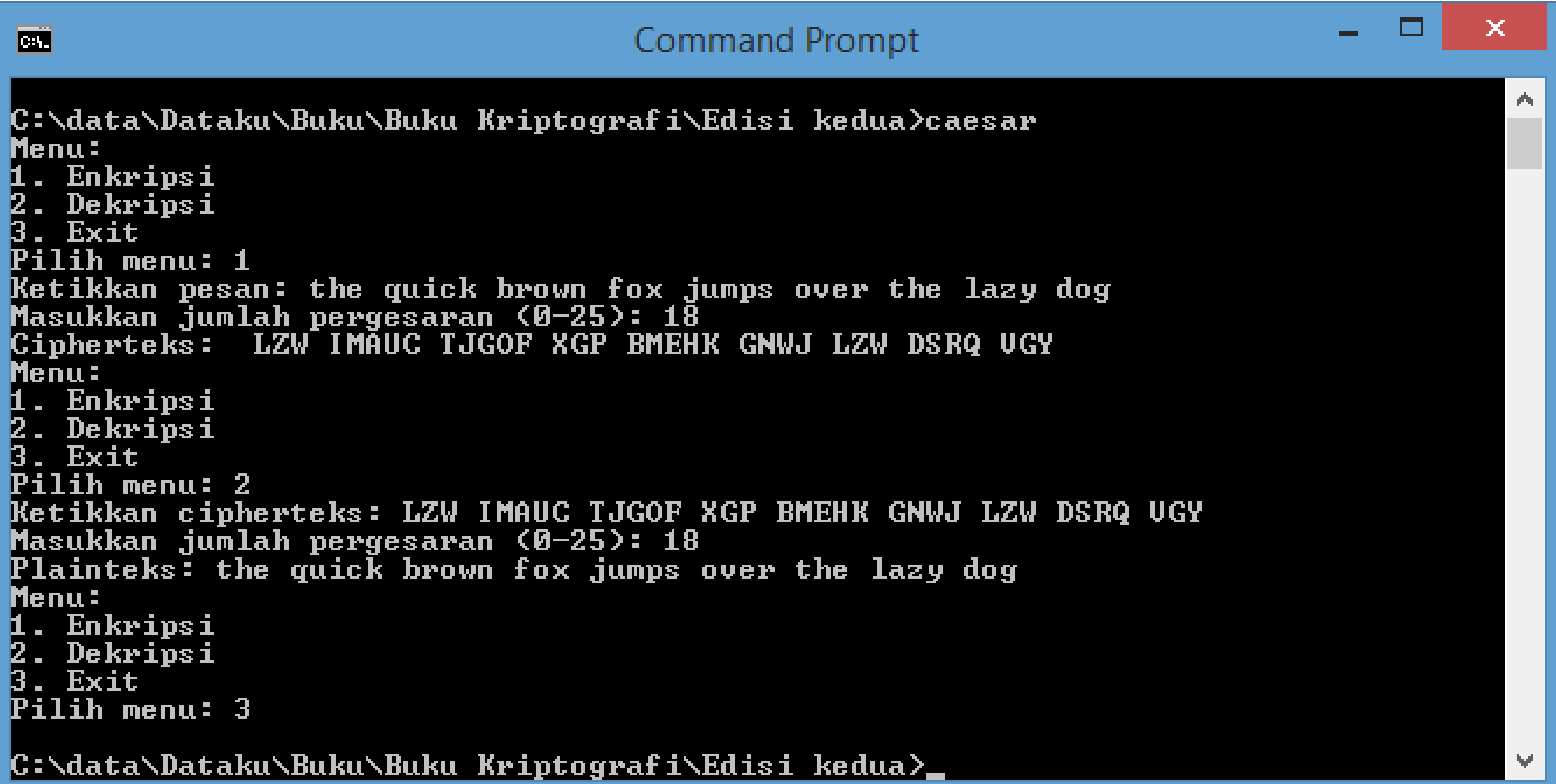
\includegraphics[width=170.10mm,height=215.62mm]{../../images/llm/page_023_img_01.png}%
\end{textblock*}

\end{document}
